\chapter{Supplemental Statistical Tables}
\label{appendix:results}

\section{Simulated Data}

\subsection{Volume Registration: Power Thresholds}

\begin{table}[]
\centering
\caption{Results from the t-tests comparing the counts for the numbers of images meeting the FD, DVARS, and FD and DVARS thresholds for sequence type $S_1$ and sequence type $S_2$.}
\label{tab:spectr-power-ttest}
\begin{tabular}{|c|c|c|c|}
\hline
\textbf{Sequence Type 1 ($S_1$)} &
  \textbf{Original} &
  \textbf{Original} &
  \textbf{\begin{tabular}[c]{@{}c@{}}Traditionally \\ Registered\end{tabular}} \\ \hline
\textbf{Sequence Type 2 ($S_2$)} &
  \textbf{\begin{tabular}[c]{@{}c@{}}Traditionally\\ Registered\end{tabular}} &
  \textbf{\begin{tabular}[c]{@{}c@{}}DAG\\ Registered\end{tabular}} &
  \textbf{\begin{tabular}[c]{@{}c@{}}DAG\\ Registered\end{tabular}} \\ \hline
\begin{tabular}[c]{@{}c@{}}P($S_1$ and $S_2$ have \\ same FD counts)\end{tabular} &
  1.05 E -16 &
  4.49 E -11 &
  0.127 \\ \hline
\begin{tabular}[c]{@{}c@{}}P($S_1$ and $S_2$ have \\ same DVARS counts)\end{tabular} &
  0.941 &
  0.941 &
  1.0 \\ \hline
\begin{tabular}[c]{@{}c@{}}P($S_1$ and $S_2$ have \\ same FD and DVARS counts)\end{tabular} &
  0.590 &
  0.486 &
  0.872 \\ \hline
\end{tabular}
\end{table}

\begin{table}[]
\centering
\caption{The number of subjects whose sequences of types $S_1$ and $S_2$ had different FD distributions.}
\label{tab:spectr-fd-kstest}
\begin{tabular}{|c|c|c|c|}
\hline
\textbf{\begin{tabular}[c]{@{}c@{}}\# Sequences \\ Type 1 ($S_1$)\end{tabular}} &
  \textbf{\begin{tabular}[c]{@{}c@{}}\# Sequences \\ Type 2 ($S_2$)\end{tabular}} &
  \textbf{\begin{tabular}[c]{@{}c@{}}\# Sequences \\ p \textless 0.05\end{tabular}} &
  \textbf{\begin{tabular}[c]{@{}c@{}}\# Sequences \\ p \textless 0.005\end{tabular}} \\ \hline
Original                                                            & \begin{tabular}[c]{@{}c@{}}Traditionally\\ Registered\end{tabular} & 90 & 90 \\ \hline
Original                                                            & \begin{tabular}[c]{@{}c@{}}DAG\\ Registered\end{tabular}           & 90 & 90 \\ \hline
\begin{tabular}[c]{@{}c@{}}Traditionally \\ Registered\end{tabular} & \begin{tabular}[c]{@{}c@{}}DAG\\ Registered\end{tabular}           & 40 & 27 \\ \hline
\end{tabular}
\end{table}

\begin{table}[]
\centering
\caption{The number of subjects whose sequences of types $S_1$ and $S_2$ had different DVARS distributions.}
\label{tab:spectr-dvars-kstest}
\begin{tabular}{|c|c|c|c|}
\hline
\textbf{\begin{tabular}[c]{@{}c@{}}\# Sequences \\ Type 1 ($S_1$)\end{tabular}} &
  \textbf{\begin{tabular}[c]{@{}c@{}}\# Sequences \\ Type 2 ($S_2$)\end{tabular}} &
  \textbf{\begin{tabular}[c]{@{}c@{}}\# Sequences \\ p \textless 0.05\end{tabular}} &
  \textbf{\begin{tabular}[c]{@{}c@{}}\# Sequences \\ p \textless 0.005\end{tabular}} \\ \hline
Original                                                            & \begin{tabular}[c]{@{}c@{}}Traditionally\\ Registered\end{tabular} & 90 & 90 \\ \hline
Original                                                            & \begin{tabular}[c]{@{}c@{}}DAG\\ Registered\end{tabular}           & 90 & 90 \\ \hline
\begin{tabular}[c]{@{}c@{}}Traditionally \\ Registered\end{tabular} & \begin{tabular}[c]{@{}c@{}}DAG\\ Registered\end{tabular}           & 3  & 0  \\ \hline
\end{tabular}
\end{table}

\clearpage

\subsection{Volume Registration: Sequence Duration Motion}

\begin{table}[]
\centering
\caption{Results of t-tests comparing the descriptive statistics of the correlation ratio matrices for the simulated data.}
\label{tab:spectr-cr-ttest}
\begin{tabular}{|c|c|c|c|}
\hline
\textbf{Sequence Type 1 ($S_1$)} &
  \textbf{Original} &
  \textbf{Original} &
  \textbf{\begin{tabular}[c]{@{}c@{}}Traditionally \\ Registered\end{tabular}} \\ \hline
\textbf{Sequence Type 2 ($S_2$)} &
  \textbf{\begin{tabular}[c]{@{}c@{}}Traditionally\\ Registered\end{tabular}} &
  \textbf{\begin{tabular}[c]{@{}c@{}}DAG\\ Registered\end{tabular}} &
  \textbf{\begin{tabular}[c]{@{}c@{}}DAG\\ Registered\end{tabular}} \\ \hline
\begin{tabular}[c]{@{}c@{}}P($S_1$ and $S_2$ \\ have same minimums)\end{tabular} &
  0.3487 &
  0.3407 &
  0.9821 \\ \hline
\begin{tabular}[c]{@{}c@{}}P($S_1$ and $S_2$ \\ have same 1st quartile)\end{tabular} &
  9.750 E -113 &
  1.246 E -112 &
  0.8019 \\ \hline
\begin{tabular}[c]{@{}c@{}}P($S_1$ and $S_2$ \\ have same medians)\end{tabular} &
  5.288 E -88 &
  5.409 E -88 &
  0.9997 \\ \hline
\begin{tabular}[c]{@{}c@{}}P($S_1$ and $S_2$ \\ have same 3rd quartiles)\end{tabular} &
  6.534 E -81 &
  6.730 E -81 &
  0.9577 \\ \hline
\begin{tabular}[c]{@{}c@{}}P($S_1$ and $S_2$ \\ have same maximums)\end{tabular} &
  2.536 E -98 &
  6.180 E -103 &
  0.4068 \\ \hline
\end{tabular}
\end{table}

\begin{table}[]
\centering
\caption{Results of t-tests comparing the descriptive statistics of the Dice matrices for the simulated data.}
\label{tab:spectr-dice-ttest}
\begin{tabular}{|c|c|c|c|}
\hline
\textbf{Sequence Type 1 ($S_1$)} &
  \textbf{Original} &
  \textbf{Original} &
  \textbf{\begin{tabular}[c]{@{}c@{}}Traditionally \\ Registered\end{tabular}} \\ \hline
\textbf{Sequence Type 2 ($S_2$)} &
  \textbf{\begin{tabular}[c]{@{}c@{}}Traditionally\\ Registered\end{tabular}} &
  \textbf{\begin{tabular}[c]{@{}c@{}}DAG\\ Registered\end{tabular}} &
  \textbf{\begin{tabular}[c]{@{}c@{}}DAG\\ Registered\end{tabular}} \\ \hline
\begin{tabular}[c]{@{}c@{}}P($S_1$ and $S_2$ \\ have same minimums)\end{tabular} &
  9.976 E -105 &
  2.520 E -110 &
  0.3778 \\ \hline
\begin{tabular}[c]{@{}c@{}}P($S_1$ and $S_2$ \\ have same 1st quartile)\end{tabular} &
  5.225 E -93 &
  5.582 E -93 &
  0.931 \\ \hline
\begin{tabular}[c]{@{}c@{}}P($S_1$ and $S_2$ \\ have same medians)\end{tabular} &
  1.988 E -104 &
  2.158 E -104 &
  0.9578 \\ \hline
\begin{tabular}[c]{@{}c@{}}P($S_1$ and $S_2$ \\ have same 3rd quartiles)\end{tabular} &
  1.679 E -131 &
  2.190 E -131 &
  0.842 \\ \hline
\begin{tabular}[c]{@{}c@{}}P($S_1$ and $S_2$ \\ have same maximums)\end{tabular} &
  1.0 &
  1.0 &
  1.0 \\ \hline
\end{tabular}
\end{table}

\clearpage

\begin{table}[]
\centering
\caption{Results of t-tests comparing the descriptive statistics of the MI matrices for the simulated data.}
\label{tab:spectr-mi-ttest}
\begin{tabular}{|c|c|c|c|}
\hline
\textbf{Sequence Type 1 ($S_1$)} &
  \textbf{Original} &
  \textbf{Original} &
  \textbf{\begin{tabular}[c]{@{}c@{}}Traditionally \\ Registered\end{tabular}} \\ \hline
\textbf{Sequence Type 2 ($S_2$)} &
  \textbf{\begin{tabular}[c]{@{}c@{}}Traditionally\\ Registered\end{tabular}} &
  \textbf{\begin{tabular}[c]{@{}c@{}}DAG\\ Registered\end{tabular}} &
  \textbf{\begin{tabular}[c]{@{}c@{}}DAG\\ Registered\end{tabular}} \\ \hline
\begin{tabular}[c]{@{}c@{}}P($S_1$ and $S_2$ \\ have same minimums)\end{tabular} &
  5.016 E -114 &
  6.328 E -126 &
  0.5397 \\ \hline
\begin{tabular}[c]{@{}c@{}}P($S_1$ and $S_2$ \\ have same 1st quartile)\end{tabular} &
  4.68 E -105 &
  7.90 E -105 &
  0.995 \\ \hline
\begin{tabular}[c]{@{}c@{}}P($S_1$ and $S_2$ \\ have same medians)\end{tabular} &
  1.65 E -97 &
  3.57 E -97 &
  0.994 \\ \hline
\begin{tabular}[c]{@{}c@{}}P($S_1$ and $S_2$ \\ have same 3rd quartiles)\end{tabular} &
  1.065 E -84 &
  2.374 E -84 &
  0.974 \\ \hline
\begin{tabular}[c]{@{}c@{}}P($S_1$ and $S_2$ \\ have same maximums)\end{tabular} &
  0.00473 &
  0.00794 &
  0.8761 \\ \hline
\end{tabular}
\end{table}

\clearpage

\section{Preadolescent Cohort}

\subsection{Volume Registration: Power Thresholds}

\begin{table}[]
\centering
\caption{Results from the t-tests comparing the counts for the numbers of images meeting the FD, DVARS, and FD and DVARS thresholds for sequence type $S_1$ and sequence type $S_2$.}
\label{tab:pread-power-ttest}
\begin{tabular}{|c|c|c|c|}
\hline
\textbf{Sequence Type 1 ($S_1$)} &
  \textbf{Original} &
  \textbf{Original} &
  \textbf{\begin{tabular}[c]{@{}c@{}}Traditionally \\ Registered\end{tabular}} \\ \hline
\textbf{Sequence Type 2 ($S_2$)} &
  \textbf{\begin{tabular}[c]{@{}c@{}}Traditionally\\ Registered\end{tabular}} &
  \textbf{\begin{tabular}[c]{@{}c@{}}DAG\\ Registered\end{tabular}} &
  \textbf{\begin{tabular}[c]{@{}c@{}}DAG\\ Registered\end{tabular}} \\ \hline
\begin{tabular}[c]{@{}c@{}}P($S_1$ and $S_2$ have \\ same FD counts)\end{tabular} &
  2.81 E -16 &
  2.35 E -16 &
  0.998 \\ \hline
\begin{tabular}[c]{@{}c@{}}P($S_1$ and $S_2$ have \\ same DVARS counts)\end{tabular} &
  9.43 E -12 &
  5.30 E -12 &
  0.950 \\ \hline
\begin{tabular}[c]{@{}c@{}}P($S_1$ and $S_2$ have \\ same FD and DVARS counts)\end{tabular} &
  1.12 E -11 &
  5.60 E -12 &
  0.938 \\ \hline
\end{tabular}
\end{table}


\clearpage

\subsection{Volume Registration: Sequence Duration Motion}

\begin{table}[]
\centering
\caption{Results of t-tests comparing the descriptive statistics of the Dice matrices for the preadolescent data.}
\label{tab:preads-dice-ttest}
\begin{tabular}{|c|c|c|c|}
\hline
\textbf{Sequence Type 1 ($S_1$)} &
  \textbf{Original} &
  \textbf{Original} &
  \textbf{\begin{tabular}[c]{@{}c@{}}Traditionally \\ Registered\end{tabular}} \\ \hline
\textbf{Sequence Type 2 ($S_2$)} &
  \textbf{\begin{tabular}[c]{@{}c@{}}Traditionally\\ Registered\end{tabular}} &
  \textbf{\begin{tabular}[c]{@{}c@{}}DAG\\ Registered\end{tabular}} &
  \textbf{\begin{tabular}[c]{@{}c@{}}DAG\\ Registered\end{tabular}} \\ \hline
\begin{tabular}[c]{@{}c@{}}P($S_1$ and $S_2$ \\ have same minimums)\end{tabular} &
  0.770 &
  0.695 &
  0.916 \\ \hline
\begin{tabular}[c]{@{}c@{}}P($S_1$ and $S_2$ \\ have same 1st quartile)\end{tabular} &
  0.976 &
  0.906 &
  0.880 \\ \hline
\begin{tabular}[c]{@{}c@{}}P($S_1$ and $S_2$ \\ have same medians)\end{tabular} &
  0.883 &
  0.562 &
  0.643 \\ \hline
\begin{tabular}[c]{@{}c@{}}P($S_1$ and $S_2$ \\ have same 3rd quartiles)\end{tabular} &
  0.000343 &
  0.000586 &
  0.390 \\ \hline
\begin{tabular}[c]{@{}c@{}}P($S_1$ and $S_2$ \\ have same maximums)\end{tabular} &
  1.0 &
  1.0 &
  1.0 \\ \hline
\end{tabular}
\end{table}

\begin{table}[]
\centering
\caption{Results of t-tests comparing the descriptive statistics of the MI matrices for the preadolescent data.}
\label{tab:preads-mi-ttest}
\begin{tabular}{|c|c|c|c|}
\hline
\textbf{Sequence Type 1 ($S_1$)} &
  \textbf{Original} &
  \textbf{Original} &
  \textbf{\begin{tabular}[c]{@{}c@{}}Traditionally \\ Registered\end{tabular}} \\ \hline
\textbf{Sequence Type 2 ($S_2$)} &
  \textbf{\begin{tabular}[c]{@{}c@{}}Traditionally\\ Registered\end{tabular}} &
  \textbf{\begin{tabular}[c]{@{}c@{}}DAG\\ Registered\end{tabular}} &
  \textbf{\begin{tabular}[c]{@{}c@{}}DAG\\ Registered\end{tabular}} \\ \hline
\begin{tabular}[c]{@{}c@{}}P($S_1$ and $S_2$ \\ have same minimums)\end{tabular} &
  0.624 &
  0.718 &
  0.896 \\ \hline
\begin{tabular}[c]{@{}c@{}}P($S_1$ and $S_2$ \\ have same 1st quartile)\end{tabular} &
  0.489 &
  0.497 &
  0.992 \\ \hline
\begin{tabular}[c]{@{}c@{}}P($S_1$ and $S_2$ \\ have same medians)\end{tabular} &
  0.364 &
  0.324 &
  0.928 \\ \hline
\begin{tabular}[c]{@{}c@{}}P($S_1$ and $S_2$ \\ have same 3rd quartiles)\end{tabular} &
  0.121 &
  0.0882 &
  0.851 \\ \hline
\begin{tabular}[c]{@{}c@{}}P($S_1$ and $S_2$ \\ have same maximums)\end{tabular} &
  0.946 &
  0.932 &
  0.987 \\ \hline
\end{tabular}
\end{table}

\clearpage

%-----------------------------------------------------------------
\section{Neonatal Cohort}

\begin{table}[]
\centering
\caption{Results from the t-tests comparing the counts for the numbers of images meeting the FD, DVARS, and FD and DVARS thresholds for sequence type $S_1$ and sequence type $S_2$.}
\label{tab:neonate-power-ttest}
\begin{tabular}{|c|c|c|c|}
\hline
\textbf{Sequence Type 1 ($S_1$)} &
  \textbf{Original} &
  \textbf{Original} &
  \textbf{\begin{tabular}[c]{@{}c@{}}Traditionally \\ Registered\end{tabular}} \\ \hline
\textbf{Sequence Type 2 ($S_2$)} &
  \textbf{\begin{tabular}[c]{@{}c@{}}Traditionally\\ Registered\end{tabular}} &
  \textbf{\begin{tabular}[c]{@{}c@{}}DAG\\ Registered\end{tabular}} &
  \textbf{\begin{tabular}[c]{@{}c@{}}DAG\\ Registered\end{tabular}} \\ \hline
\begin{tabular}[c]{@{}c@{}}P($S_1$ and $S_2$ have \\ same FD counts)\end{tabular} &
  0.0110 &
  0.00813 &
  0.924 \\ \hline
\begin{tabular}[c]{@{}c@{}}P($S_1$ and $S_2$ have \\ same DVARS counts)\end{tabular} &
  0.00163 &
  0.000942 &
  0.880 \\ \hline
\begin{tabular}[c]{@{}c@{}}P($S_1$ and $S_2$ have \\ same FD and DVARS counts)\end{tabular} &
  0.00779 &
  0.00475 &
  0.879 \\ \hline
\end{tabular}
\end{table}

\subsection{Volume Registration: Sequence Duration Motion}

\begin{table}[]
\centering
\caption{Results of t-tests comparing the descriptive statistics of the Dice matrices for the neonatal cohort.}
\label{tab:neonates-dice-ttest}
\begin{tabular}{|c|c|c|c|}
\hline
\textbf{Sequence Type 1 ($S_1$)} &
  \textbf{Original} &
  \textbf{Original} &
  \textbf{\begin{tabular}[c]{@{}c@{}}Traditionally \\ Registered\end{tabular}} \\ \hline
\textbf{Sequence Type 2 ($S_2$)} &
  \textbf{\begin{tabular}[c]{@{}c@{}}Traditionally\\ Registered\end{tabular}} &
  \textbf{\begin{tabular}[c]{@{}c@{}}DAG\\ Registered\end{tabular}} &
  \textbf{\begin{tabular}[c]{@{}c@{}}DAG\\ Registered\end{tabular}} \\ \hline
\begin{tabular}[c]{@{}c@{}}P($S_1$ and $S_2$ \\ have same minimums)\end{tabular} &
  0.523 &
  0.542 &
  0.977 \\ \hline
\begin{tabular}[c]{@{}c@{}}P($S_1$ and $S_2$ \\ have same 1st quartile)\end{tabular} &
  0.468 &
  0.515 &
  0.933 \\ \hline
\begin{tabular}[c]{@{}c@{}}P($S_1$ and $S_2$ \\ have same medians)\end{tabular} &
  0.329 &
  0.292 &
  0.937 \\ \hline
\begin{tabular}[c]{@{}c@{}}P($S_1$ and $S_2$ \\ have same 3rd quartiles)\end{tabular} &
  0.149 &
  0.115 &
  0.890 \\ \hline
\begin{tabular}[c]{@{}c@{}}P($S_1$ and $S_2$ \\ have same maximums)\end{tabular} &
  1.0 &
  1.0 &
  1.0 \\ \hline
\end{tabular}
\end{table}

\begin{table}[]
\centering
\caption{Results of t-tests comparing the descriptive statistics of the MI matrices for the neonatal data.}
\label{tab:neonates-mi-ttest}
\begin{tabular}{|c|c|c|c|}
\hline
\textbf{Sequence Type 1 ($S_1$)} &
  \textbf{Original} &
  \textbf{Original} &
  \textbf{\begin{tabular}[c]{@{}c@{}}Traditionally \\ Registered\end{tabular}} \\ \hline
\textbf{Sequence Type 2 ($S_2$)} &
  \textbf{\begin{tabular}[c]{@{}c@{}}Traditionally\\ Registered\end{tabular}} &
  \textbf{\begin{tabular}[c]{@{}c@{}}DAG\\ Registered\end{tabular}} &
  \textbf{\begin{tabular}[c]{@{}c@{}}DAG\\ Registered\end{tabular}} \\ \hline
\begin{tabular}[c]{@{}c@{}}P($S_1$ and $S_2$ \\ have same minimums)\end{tabular} &
  0.853 &
  0.874 &
  0.978 \\ \hline
\begin{tabular}[c]{@{}c@{}}P($S_1$ and $S_2$ \\ have same 1st quartile)\end{tabular} &
  0.794 &
  0.809 &
  0.985 \\ \hline
\begin{tabular}[c]{@{}c@{}}P($S_1$ and $S_2$ \\ have same medians)\end{tabular} &
  0.762 &
  0.758 &
  0.996 \\ \hline
\begin{tabular}[c]{@{}c@{}}P($S_1$ and $S_2$ \\ have same 3rd quartiles)\end{tabular} &
  0.755 &
  0.743 &
  0.987 \\ \hline
\begin{tabular}[c]{@{}c@{}}P($S_1$ and $S_2$ \\ have same maximums)\end{tabular} &
  0.956 &
  0.938 &
  0.982 \\ \hline
\end{tabular}
\end{table}

\section{Fetal Cohort}

\subsection{Brain}

\subsubsection{Volume Registration: Power Thresholds}

\begin{table}[]
\centering
\caption{Results from the t-tests comparing the counts for the numbers of images meeting the FD, DVARS, and FD and DVARS thresholds for fetal brain sequence type $S_1$ and sequence type $S_2$.}
\label{tab:fetal-brain-power-ttest}
\begin{tabular}{|c|c|c|c|}
\hline
\textbf{Sequence Type 1 ($S_1$)} &
  \textbf{Original} &
  \textbf{Original} &
  \textbf{\begin{tabular}[c]{@{}c@{}}Traditionally \\ Registered\end{tabular}} \\ \hline
\textbf{Sequence Type 2 ($S_2$)} &
  \textbf{\begin{tabular}[c]{@{}c@{}}Traditionally\\ Registered\end{tabular}} &
  \textbf{\begin{tabular}[c]{@{}c@{}}DAG\\ Registered\end{tabular}} &
  \textbf{\begin{tabular}[c]{@{}c@{}}DAG\\ Registered\end{tabular}} \\ \hline
\begin{tabular}[c]{@{}c@{}}P($S_1$ and $S_2$ have \\ same FD counts)\end{tabular} &
  0.811 &
  0.926 &
  0.883 \\ \hline
\begin{tabular}[c]{@{}c@{}}P($S_1$ and $S_2$ have \\ same DVARS counts)\end{tabular} &
  0.159 &
  1.0 &
  0.159 \\ \hline
\begin{tabular}[c]{@{}c@{}}P($S_1$ and $S_2$ have \\ same FD and DVARS counts)\end{tabular} &
  0.159 &
  1.0 &
  0.159 \\ \hline
\end{tabular}
\end{table}

\subsubsection{Volume Registration: Sequence Duration Motion}

\begin{table}[]
\centering
\caption{Results of t-tests comparing the descriptive statistics of the Dice matrices for the fetal brain data.}
\label{tab:fetal-brain-dice-ttest}
\begin{tabular}{|c|c|c|c|}
\hline
\textbf{Sequence Type 1 ($S_1$)} &
  \textbf{Original} &
  \textbf{Original} &
  \textbf{\begin{tabular}[c]{@{}c@{}}Traditionally \\ Registered\end{tabular}} \\ \hline
\textbf{Sequence Type 2 ($S_2$)} &
  \textbf{\begin{tabular}[c]{@{}c@{}}Traditionally\\ Registered\end{tabular}} &
  \textbf{\begin{tabular}[c]{@{}c@{}}DAG\\ Registered\end{tabular}} &
  \textbf{\begin{tabular}[c]{@{}c@{}}DAG\\ Registered\end{tabular}} \\ \hline
\begin{tabular}[c]{@{}c@{}}P($S_1$ and $S_2$ \\ have same minimums)\end{tabular} &
  0.259 &
  0.932 &
  0.289 \\ \hline
\begin{tabular}[c]{@{}c@{}}P($S_1$ and $S_2$ \\ have same 1st quartile)\end{tabular} &
  0.254 &
  0.996 &
  0.252 \\ \hline
\begin{tabular}[c]{@{}c@{}}P($S_1$ and $S_2$ \\ have same medians)\end{tabular} &
  0.658 &
  0.970 &
  0.686 \\ \hline
\begin{tabular}[c]{@{}c@{}}P($S_1$ and $S_2$ \\ have same 3rd quartiles)\end{tabular} &
  0.973 &
  0.921 &
  0.896 \\ \hline
\begin{tabular}[c]{@{}c@{}}P($S_1$ and $S_2$ \\ have same maximums)\end{tabular} &
  1.0 &
  1.0 &
  1.0 \\ \hline
\end{tabular}
\end{table}

\begin{table}[]
\centering
\caption{Results of t-tests comparing the descriptive statistics of the MI matrices for the fetal brain data.}
\label{tab:fetal-brain-mi-ttest}
\begin{tabular}{|c|c|c|c|}
\hline
\textbf{Sequence Type 1 ($S_1$)} &
  \textbf{Original} &
  \textbf{Original} &
  \textbf{\begin{tabular}[c]{@{}c@{}}Traditionally \\ Registered\end{tabular}} \\ \hline
\textbf{Sequence Type 2 ($S_2$)} &
  \textbf{\begin{tabular}[c]{@{}c@{}}Traditionally\\ Registered\end{tabular}} &
  \textbf{\begin{tabular}[c]{@{}c@{}}DAG\\ Registered\end{tabular}} &
  \textbf{\begin{tabular}[c]{@{}c@{}}DAG\\ Registered\end{tabular}} \\ \hline
\begin{tabular}[c]{@{}c@{}}P($S_1$ and $S_2$ \\ have same minimums)\end{tabular} &
  0.673 &
  0.845 &
  0.816 \\ \hline
\begin{tabular}[c]{@{}c@{}}P($S_1$ and $S_2$ \\ have same 1st quartile)\end{tabular} &
  0.765 &
  0.963 &
  0.798 \\ \hline
\begin{tabular}[c]{@{}c@{}}P($S_1$ and $S_2$ \\ have same medians)\end{tabular} &
  0.764 &
  0.963 &
  0.798 \\ \hline
\begin{tabular}[c]{@{}c@{}}P($S_1$ and $S_2$ \\ have same 3rd quartiles)\end{tabular} &
  0.760 &
  0.959 &
  0.797 \\ \hline
\begin{tabular}[c]{@{}c@{}}P($S_1$ and $S_2$ \\ have same maximums)\end{tabular} &
  0.539 &
  0.999 &
  0.539 \\ \hline
\end{tabular}
\end{table}

\subsection{Placenta}

\subsubsection{Volume Registration: Power Thresholds}

\begin{table}[]
\centering
\caption{Results from the t-tests comparing the counts for the numbers of images meeting the FD, DVARS, and FD and DVARS thresholds for fetal placenta sequence type $S_1$ and sequence type $S_2$.}
\label{tab:fetal-placenta-power-ttest}
\begin{tabular}{|c|c|c|c|}
\hline
\textbf{Sequence Type 1 ($S_1$)} &
  \textbf{Original} &
  \textbf{Original} &
  \textbf{\begin{tabular}[c]{@{}c@{}}Traditionally \\ Registered\end{tabular}} \\ \hline
\textbf{Sequence Type 2 ($S_2$)} &
  \textbf{\begin{tabular}[c]{@{}c@{}}Traditionally\\ Registered\end{tabular}} &
  \textbf{\begin{tabular}[c]{@{}c@{}}DAG\\ Registered\end{tabular}} &
  \textbf{\begin{tabular}[c]{@{}c@{}}DAG\\ Registered\end{tabular}} \\ \hline
\begin{tabular}[c]{@{}c@{}}P($S_1$ and $S_2$ have \\ same FD counts)\end{tabular} &
  0.519 &
  0.350 &
  0.775 \\ \hline
\begin{tabular}[c]{@{}c@{}}P($S_1$ and $S_2$ have \\ same DVARS counts)\end{tabular} &
  5.38 E -6 &
  5.65 E -9 &
  0.101 \\ \hline
\begin{tabular}[c]{@{}c@{}}P($S_1$ and $S_2$ have \\ same FD and DVARS counts)\end{tabular} &
  5.18 E -6 &
  1.92 E -8 &
  0.0571 \\ \hline
\end{tabular}
\end{table}

\clearpage

\section{Characterizing Motion}

\subsection{Age Groups}

\begin{figure}[t]
	\centering
	\begin{subfigure}{0.49\textwidth}
		\centering
		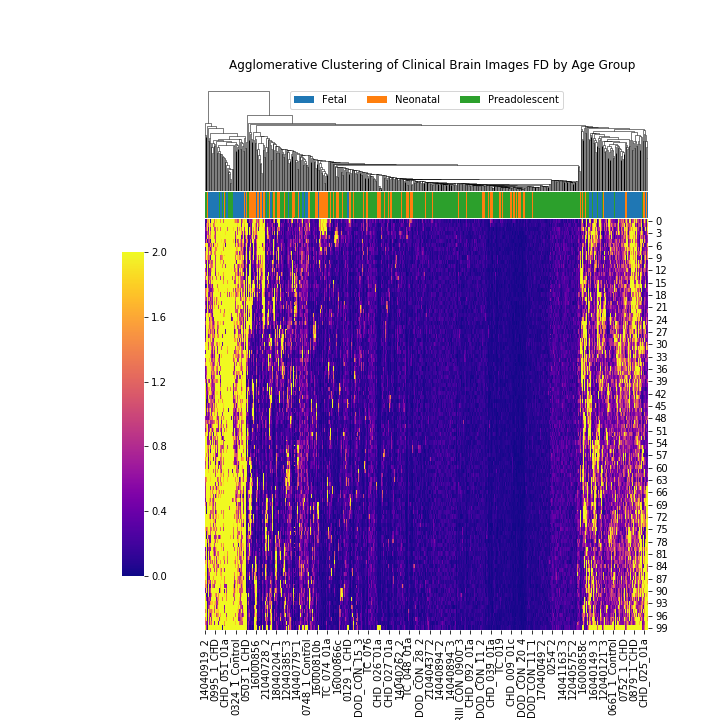
\includegraphics[width=1.0\textwidth]{6/figures/agegroup-bold-fd-sns-agg.png}
		\caption{FD}
	\end{subfigure}
	\begin{subfigure}{0.49\textwidth}
		\centering
		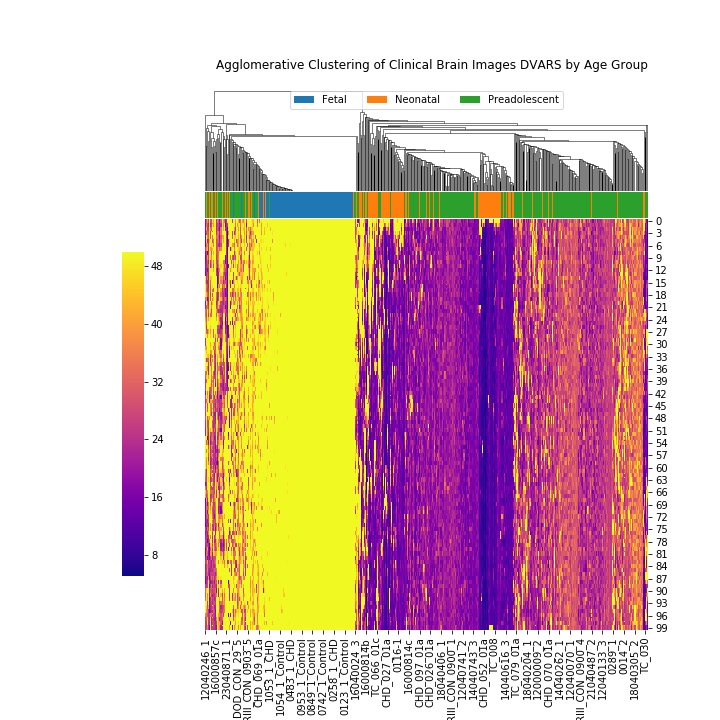
\includegraphics[width=1.0\textwidth]{6/figures/agegroup-bold-dvars-sns-agg.png}
		\caption{DVARS}
	\end{subfigure}
	
	\begin{subfigure}{0.49\textwidth}
		\centering
		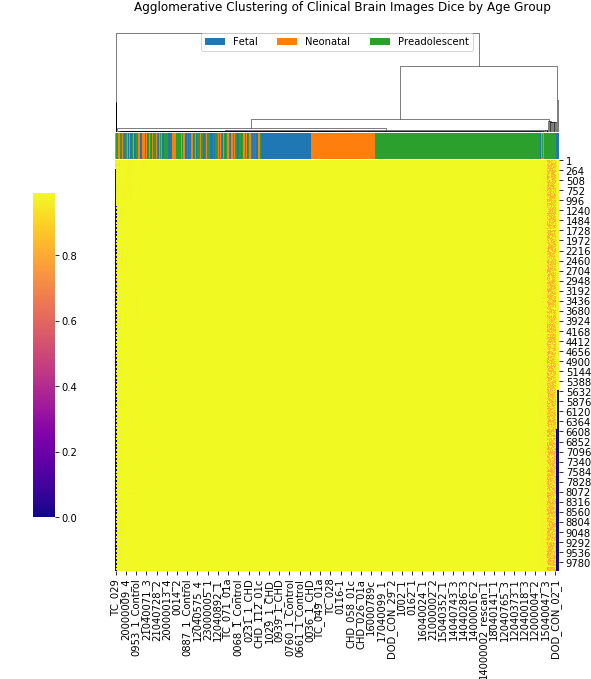
\includegraphics[width=1.0\textwidth]{6/figures/agegroup-bold-dice-sns-agg.png}
		\caption{Dice}
	\end{subfigure}
	\begin{subfigure}{0.49\textwidth}
		\centering
		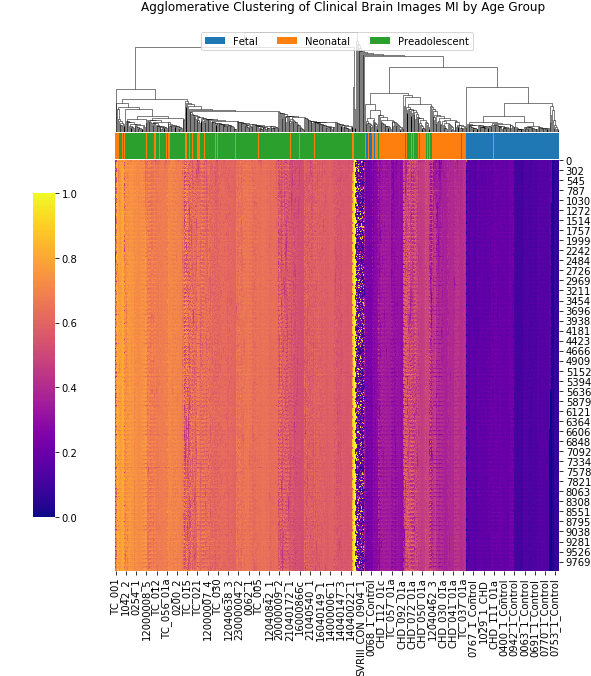
\includegraphics[width=1.0\textwidth]{6/figures/agegroup-bold-mi-sns-agg.png}
		\caption{MI}
	\end{subfigure}
\caption{The preadolescent, neonatal, and fetal images clustered by each metric using agglomerative clustering and labeled by age group.}
\label{fig:mochar-ages-sns-agg}
\end{figure}

\clearpage

\subsection{CHD and Control}

\begin{figure}[t]
	\centering
	\begin{subfigure}{0.49\textwidth}
		\centering
		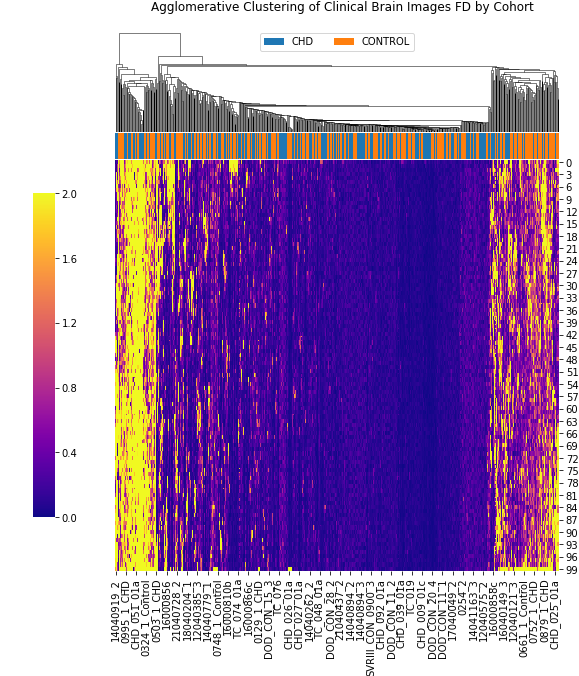
\includegraphics[width=1.0\textwidth]{6/figures/cohort-bold-fd-sns-agg.png}
		\caption{FD}
	\end{subfigure}
	\begin{subfigure}{0.49\textwidth}
		\centering
		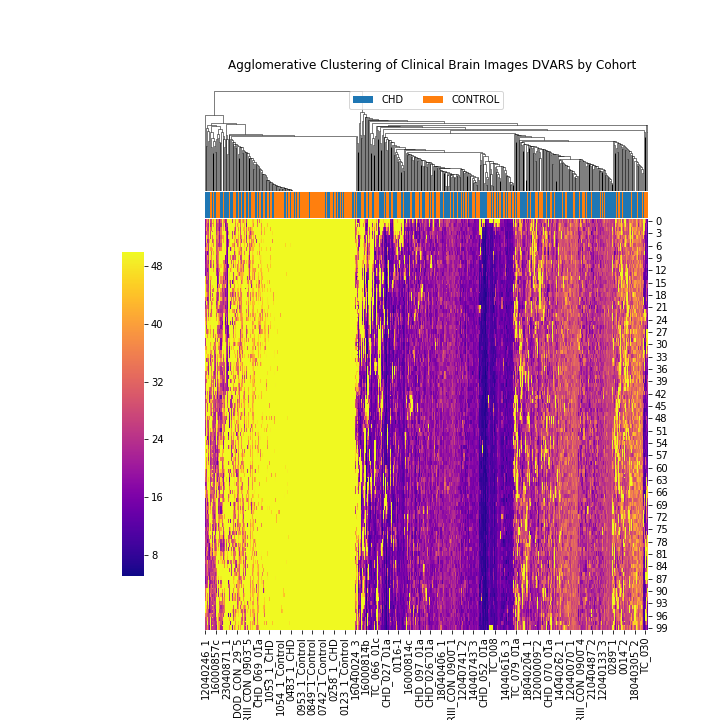
\includegraphics[width=1.0\textwidth]{6/figures/cohort-bold-dvars-sns-agg.png}
		\caption{DVARS}
	\end{subfigure}
	
	\begin{subfigure}{0.49\textwidth}
		\centering
		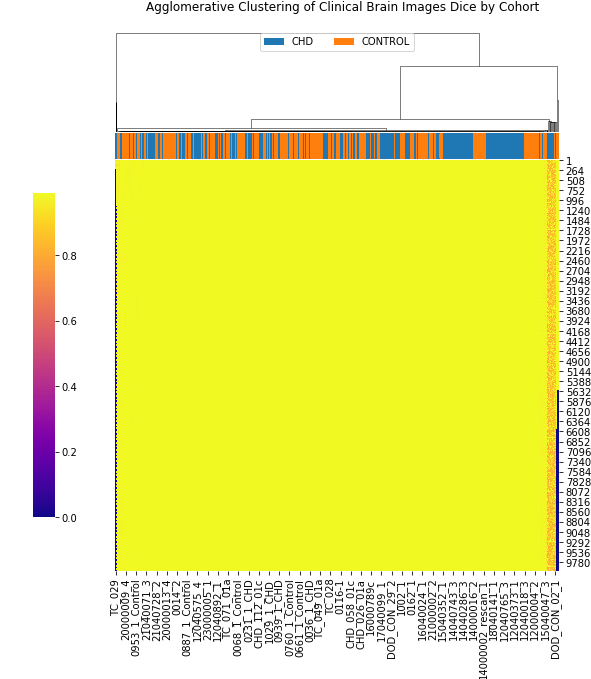
\includegraphics[width=1.0\textwidth]{6/figures/cohort-bold-dice-sns-agg.png}
		\caption{Dice}
	\end{subfigure}
	\begin{subfigure}{0.49\textwidth}
		\centering
		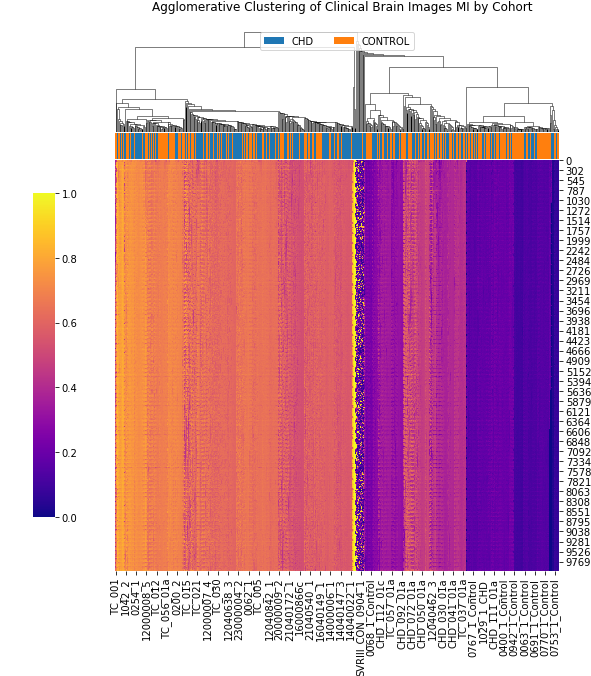
\includegraphics[width=1.0\textwidth]{6/figures/cohort-bold-mi-sns-agg.png}
		\caption{MI}
	\end{subfigure}
\caption{The preadolescent, neonatal, and fetal images clustered by each metric using agglomerative clustering and labeled by CHD/Control status.}
\label{fig:mochar-cohorts-sns-agg}
\end{figure}